\section{Analysis of Results}

We now apply the tool to the three themes set out in the Introduction.
The aim is not a complete study of any theme, but a demonstration that the visualization can surface the relevant patterns, which tabular access tends to obscure.
Each example uses complete years, since the latest year in the extract still lacks part of its final months.
As a general figure, close to 34 percent of admissions between 2015 and 2019 took place outside the patient's home municipality, so cross-border flow is substantial and worth visualizing.

\subsection{Gaps in care for a specialty}

The first theme is the gap in care, where the residents of a region must travel for a given specialty.
A municipality can be a hub for one specialty and dependent for another.
Figure~\ref{fig:gap} shows Santa Maria, a hub in the interior of Rio Grande do Sul, under two specialties in 2023.
For cardiology it received 3{,}391 admissions against 2{,}061 from its own residents, a positive balance of 1{,}330 and an export rate of 1 percent.
For gastroenterology it received 281 against 405 residents, a negative balance of 124 and an export rate of 45 percent.

Changing only the specialty filter turns Santa Maria from a blue hub reached by incoming arcs into a red municipality whose residents leave for other cities.
A pattern of this kind points a health authority to a specialty and a region that may need attention.
Because the coverage of the specialty field is uneven, the reading is most reliable where a specialty has many admissions.

\subsection{Hub cities and regional load}

The second theme is the hub city that concentrates the care of a region, where the demand it absorbs may signal overload or a bottleneck.
The ranking panel orders municipalities by their attraction balance.
Figure~\ref{fig:ranking} shows Rio Grande do Sul, where Porto Alegre attracts far more patients than any other city, followed by Passo Fundo and Santa Maria, while Viam\~{a}o, Alvorada, and Gravata\'{\i} appear among the municipalities that depend on care produced elsewhere.
A small number of hubs therefore sustains many surrounding towns.

The map shows the same balance for a single specialty.
Figure~\ref{fig:contrast} draws facial surgery for the two extremes of the ranking.
Porto Alegre is covered by incoming blue arcs from across the state and from other states, whereas Viam\~{a}o shows mostly outgoing orange arcs.
The width and direction of the arcs report the export of patients for the chosen specialty.
The per-capita metric helps separate a large hub from one that is heavily loaded for its population, which is where a bottleneck is most likely.

\subsection{Seasonal patterns}

The third theme is seasonality, and whether a peak month falls on residents or on incoming patients.
The monthly balance proves specific to each city.
Figure~\ref{fig:seasonality} shows six municipalities across the twelve months of 2021.
Vit\'{o}ria da Conquista (BA) is the most common case, where residents and incoming patients rise and fall together.
Cear\'{a}-Mirim (RN) shows both groups climbing sharply from March, a clear peak that a hospital could anticipate.

The other four cities show patterns that do not generalize.
In Muri\'{a}e (MG) the incoming patients peak several times while residents stay flat.
In Gurupi (TO) the resident and incoming peaks alternate through the year.
In Luzi\^{a}nia (GO) and Teut\^{o}nia (RS) a rise in residents coincides with a fall in incoming patients, which suggests that residents are served first when local demand grows; Teut\^{o}nia also peaks in winter.

This bears on the question of overload in peak months.
In most cities residents and incoming patients move together, so a peak is not driven by a sudden influx from outside.
In the few cities where the two diverge, the system appears to favor residents during the busiest months.
Because the behavior varies so widely, the practical value of the monthly view is local: an institution can read the curve for its own city and prepare for its own peak.

\begin{figure}[t]
  \centering
  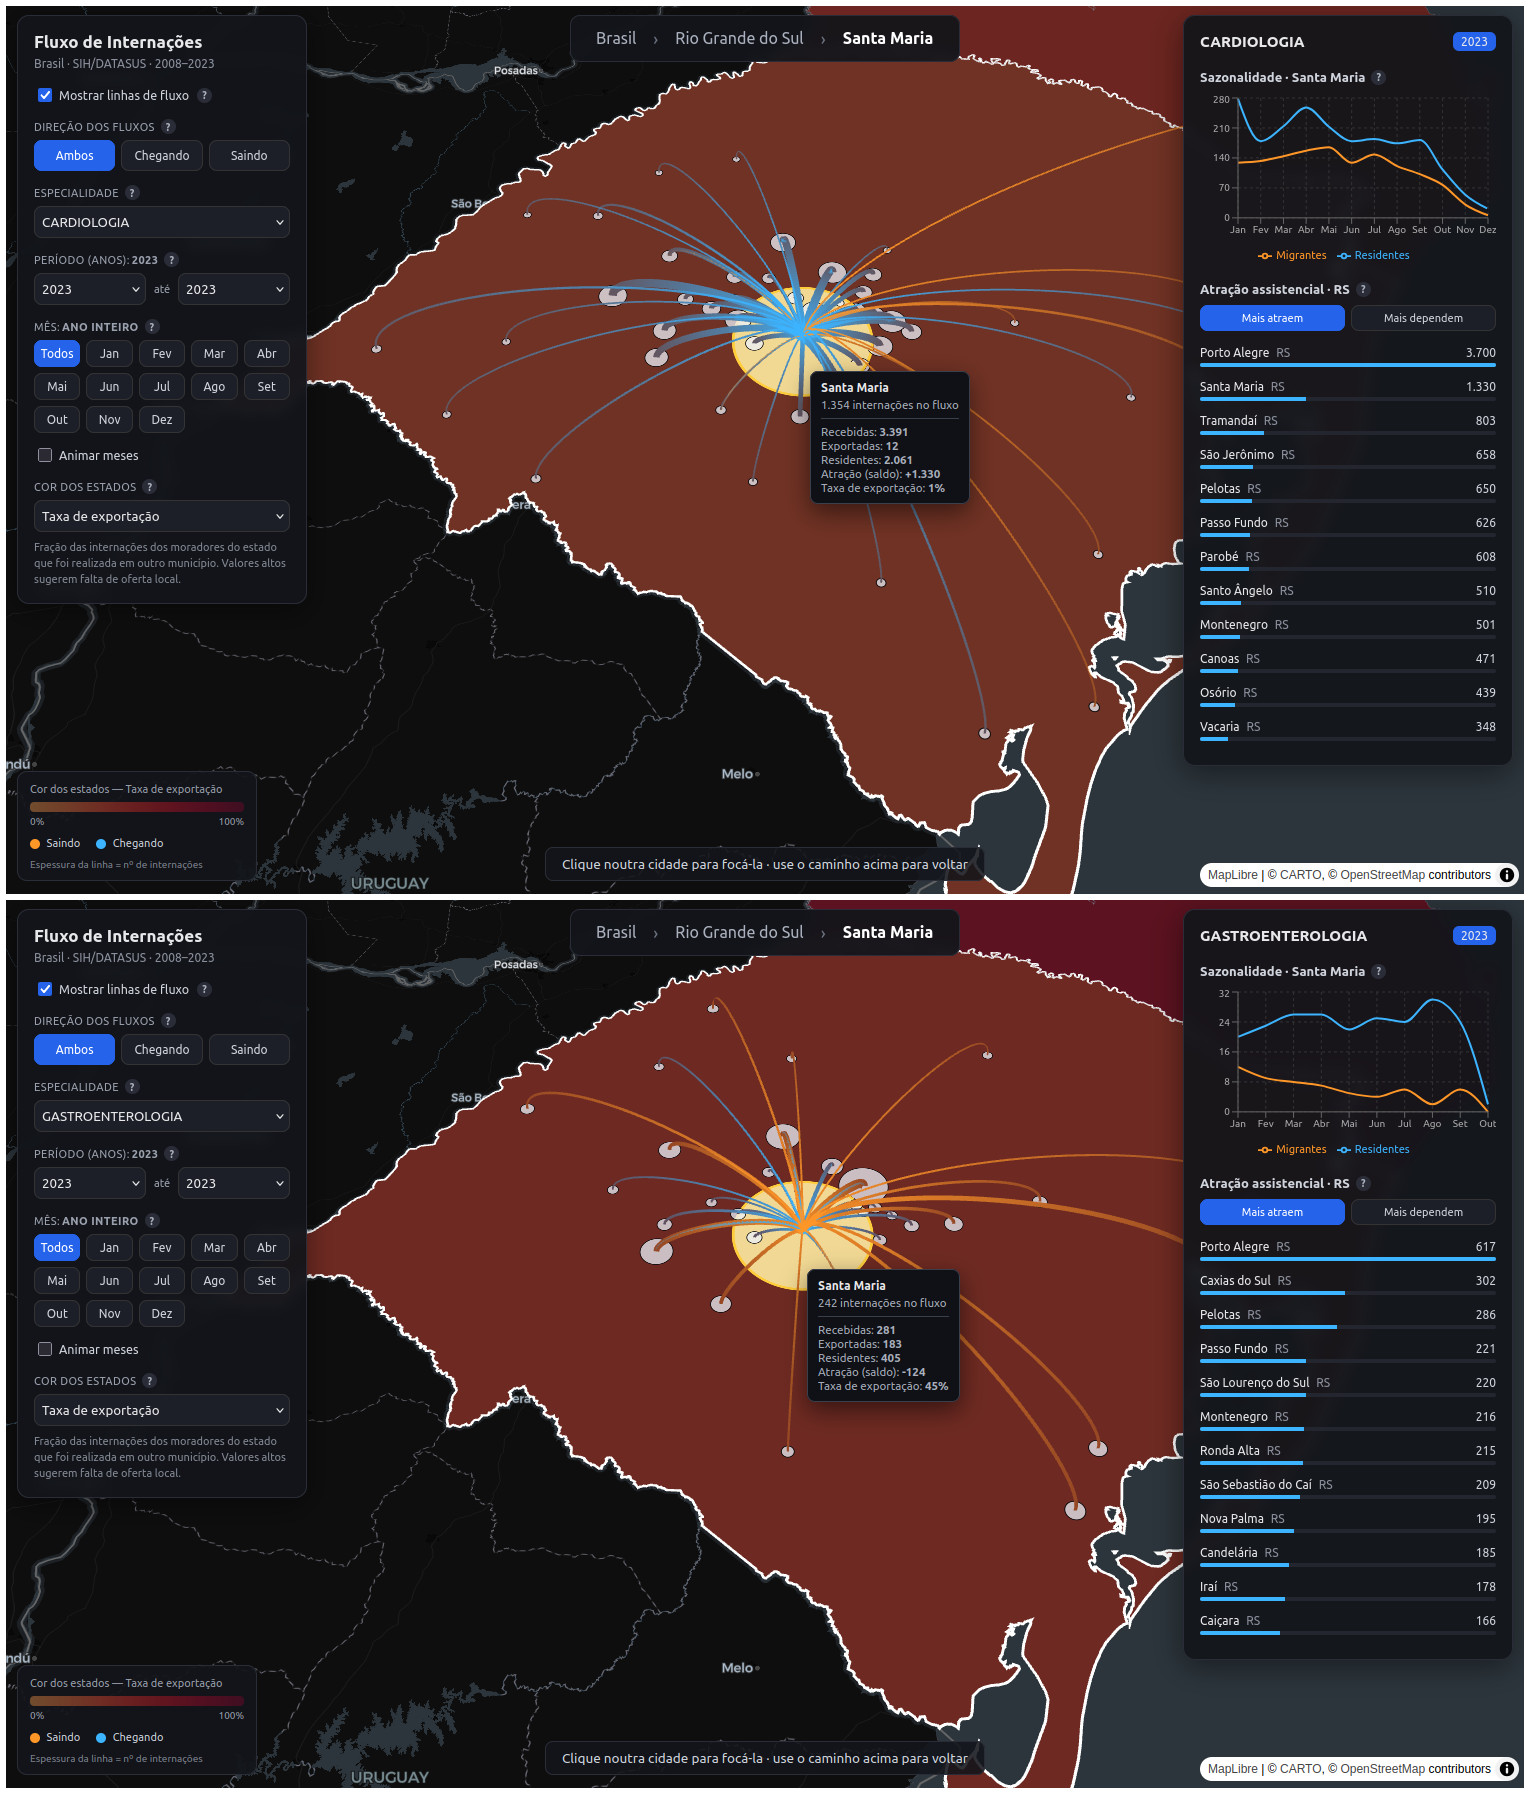
\includegraphics[width=0.95\columnwidth]{santa-maria-cardio-vs-gastro.jpeg}
  \caption{%
    Santa Maria (Rio Grande do Sul) under two specialties in 2023.
    Top: cardiology, where the city is a hub reached by incoming blue arcs (balance $+1{,}330$, export rate 1 percent).
    Bottom: gastroenterology, where its residents leave along orange arcs (balance $-124$, export rate 45 percent).
    Only the specialty filter changed between the two views.%
  }
  \label{fig:gap}
\end{figure}

\begin{figure}[t]
  \centering
  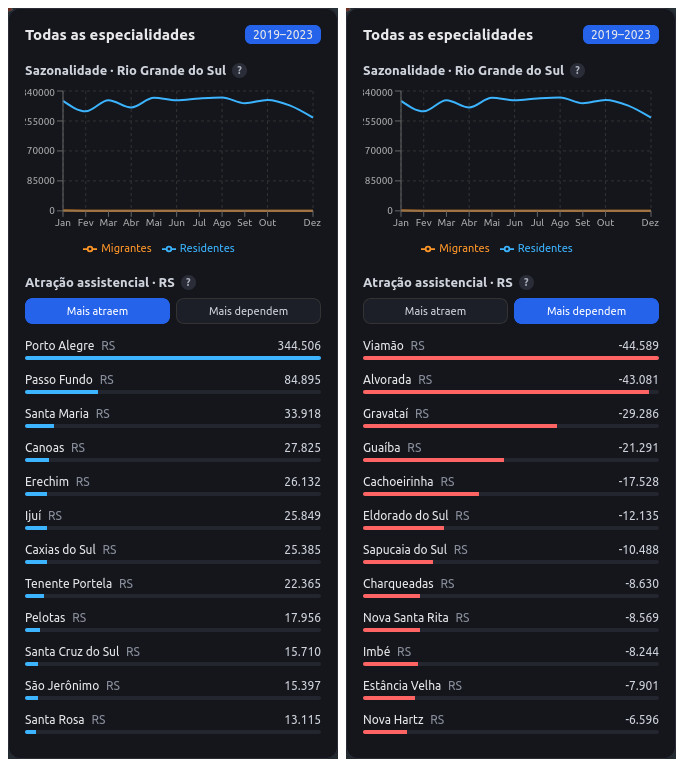
\includegraphics[width=0.92\columnwidth]{attract-vs-depend-more.jpeg}
  \caption{%
    The attraction ranking for Rio Grande do Sul, all specialties, 2019 to 2023.
    Left: the municipalities that attract the most patients, led by Porto Alegre.
    Right: the municipalities that most depend on care elsewhere, led by Viam\~{a}o.
    Bar length encodes the attraction balance, blue for positive and red for negative.%
  }
  \label{fig:ranking}
\end{figure}

\begin{figure}[t]
  \centering
  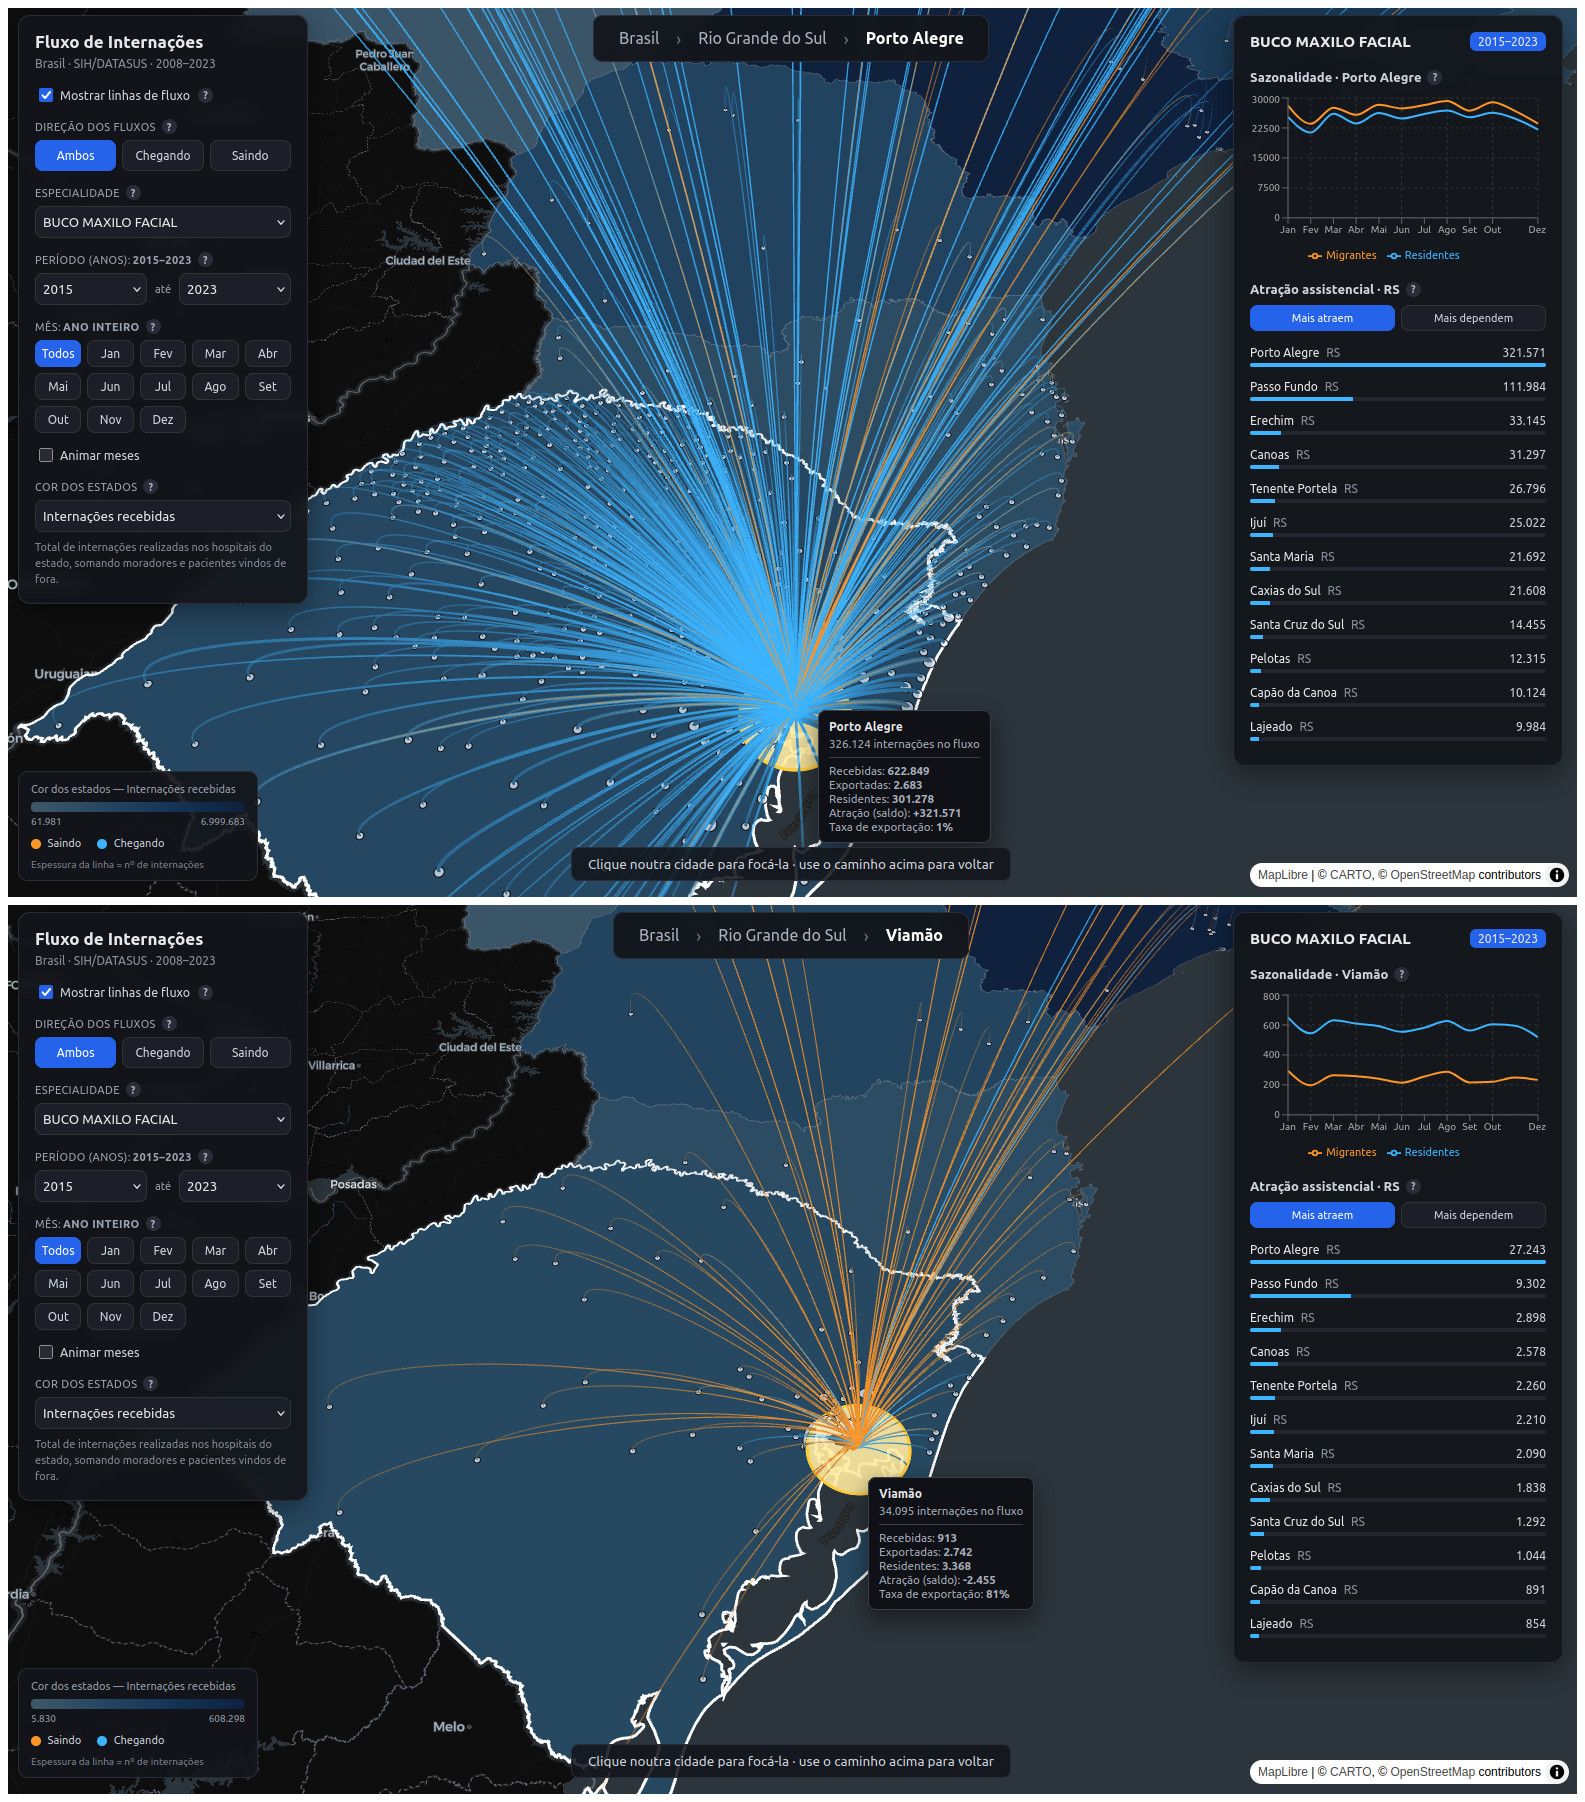
\includegraphics[width=0.92\columnwidth]{poa-vs-viamao-buco-maxilo-facial.jpeg}
  \caption{%
    City level view of two municipalities in Rio Grande do Sul for facial surgery (Buco Maxilo Facial), 2015 to 2023.
    Porto Alegre (top) is reached by many blue arcs, since patients arrive from across the state and from other states.
    Viam\~{a}o (bottom) shows mostly orange arcs, since its residents leave for other cities.
    The two are the top attracting and top dependent municipalities in the ranking of Figure~\ref{fig:ranking}.%
  }
  \label{fig:contrast}
\end{figure}

\begin{figure*}[t]
  \centering
  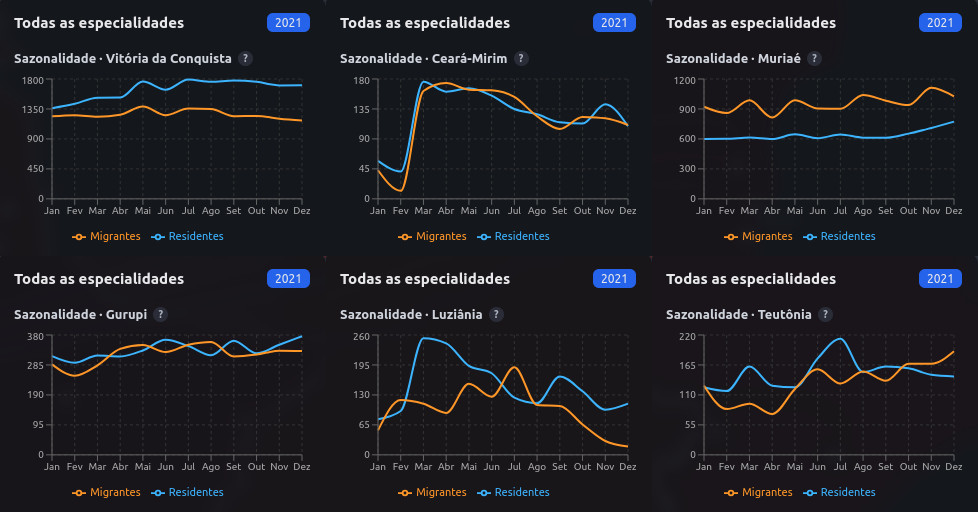
\includegraphics[width=\linewidth]{seasonal-charts.jpeg}
  \caption{%
    Monthly resident and incoming admissions for six municipalities in 2021.
    The shape of the curve changes from city to city, from residents and incoming patients moving together (Vit\'{o}ria da Conquista, BA) to shared peaks (Cear\'{a}-Mirim, RN), repeated incoming peaks (Muri\'{a}e, MG), alternating peaks (Gurupi, TO), and resident peaks that coincide with drops in incoming patients (Luzi\^{a}nia, GO and Teut\^{o}nia, RS).%
  }
  \label{fig:seasonality}
\end{figure*}
